\documentclass[11pt, a4paper, twocolumn]{article}

\usepackage[margin=0.75in, top=1in, bottom=0.9in, columnsep=0.3in]{geometry}
\usepackage{amsmath, amssymb}
\usepackage{graphicx}
\usepackage[numbers,sort&compress]{natbib}
\usepackage{booktabs}
\usepackage{float}
\usepackage{hyperref}
\usepackage{xcolor}
\usepackage{caption}
\usepackage{authblk}
\usepackage{enumitem}
\usepackage{microtype}
\usepackage{titlesec}
\usepackage{fancyhdr}

% --- Color scheme ---
\definecolor{arxivblue}{RGB}{0, 51, 102}
\definecolor{linkblue}{RGB}{10, 82, 145}
\definecolor{citegreen}{RGB}{0, 100, 60}

\hypersetup{
    colorlinks=true,
    linkcolor=linkblue,
    citecolor=citegreen,
    urlcolor=linkblue
}

% --- Caption styling ---
\captionsetup{
    font=small,
    labelfont=bf,
    labelsep=period,
    skip=6pt,
    format=plain
}

% --- Section formatting ---
\titleformat{\section}{\large\bfseries}{\thesection.}{0.5em}{}
\titleformat{\subsection}{\normalsize\bfseries}{\thesubsection}{0.5em}{}
\titleformat{\subsubsection}{\normalsize\itshape}{\thesubsubsection}{0.5em}{}
\titlespacing*{\section}{0pt}{12pt plus 2pt minus 2pt}{6pt plus 1pt}
\titlespacing*{\subsection}{0pt}{8pt plus 2pt minus 1pt}{4pt plus 1pt}
\titlespacing*{\subsubsection}{0pt}{6pt plus 2pt minus 1pt}{3pt plus 1pt}


% --- Header ---
\pagestyle{fancy}
\fancyhf{}
\fancyhead[L]{\small\textit{Preprint}}
\fancyhead[R]{\small\thepage}
\renewcommand{\headrulewidth}{0.4pt}
\fancypagestyle{plain}{
    \fancyhf{}
    \fancyhead[L]{\small\textit{Preprint}}
    \fancyhead[R]{\small\thepage}
    \renewcommand{\headrulewidth}{0.4pt}
}

% --- Compact lists ---
\setlist{nosep, leftmargin=1.5em}

% --- Title ---
\title{\vspace{-1.5em}\textbf{\large Towards a Digital Twin of the Martian Atmosphere: Deep-Learning Weather Forecasting with HEALPix-Aware Convolutions and EMARS Reanalysis}\vspace{-0.5em}}

\author[1,2]{Manmeet Singh}
\author[1]{Naveen Sudharsan}
\author[3]{Houman Owhadi}
\author[1]{Krista Soderlund}
\author[4]{Alphan Altinok}

\affil[1]{\small The University of Texas at Austin, Austin, Texas, USA}
\affil[2]{\small Western Kentucky University, Bowling Green, Kentucky, USA}
\affil[3]{\small California Institute of Technology, Pasadena, California, USA}
\affil[4]{\small NASA Jet Propulsion Laboratory, Pasadena, California, USA}

\date{\vspace{-1em}\small May 2026}

\begin{document}

\twocolumn[
\maketitle
\vspace{-0.5em}
\begin{center}\textbf{Abstract}\end{center}
\vspace{-0.5em}
{\small\noindent
Digital twins of planetary atmospheres promise fast, lightweight surrogates of expensive general circulation models for mission planning and scientific inquiry. Here we present a deep-learning weather prediction system for Mars trained on the Ensemble Mars Atmosphere Reanalysis System (EMARS) v1.0. We regrid temperature, zonal wind, and meridional wind fields across 28 vertical levels onto a hierarchical equal-area isolatitude pixelization (HEALPix) mesh at $N_\text{side} = 64$ (${\sim}110$~km resolution) and train a HEALPix-aware 2D U-Net inspired by the DLESyM architecture~\cite{wattmeyer2024} to predict the next hourly atmospheric state. The model employs custom inter-face padding that respects the topology of the 12-face HEALPix sphere, ConvNeXt residual blocks with capped GELU activations~\cite{hendrycks2016,liu2022convnext}, and a fold/unfold scheme that maps between the data pipeline format $[B, C, 12, H, W]$ and the convolution format $[B{\cdot}12, C, H, W]$. With only 4.3 million trainable parameters, the network achieves a best validation MSE of $1.58 \times 10^{-5}$ in normalized units. Recursive autoregressive rollouts remain stable and physically coherent for 24 hours, with RMSE growing monotonically from ${\sim}0.004$ at T+1\,h to ${\sim}0.029$ at T+24\,h without divergence. Compared to a baseline 3D U-Net~\cite{ronneberger2015,cicek20163d}, the HEALPix-aware architecture reduces validation loss by more than an order of magnitude while using fewer parameters. The model generates a one-hour forecast in approximately 0.5~seconds on a single GPU, offering several orders-of-magnitude speedup over the GFDL/NASA Mars GCM. These results demonstrate that parsimonious, geometry-respecting neural architectures can capture synoptic-scale Martian atmospheric dynamics and provide a foundation for operational Mars digital twins.\par}
\vspace{1.5em}
]

% ===================================================================
\section{Introduction}
% ===================================================================

Mars' thin CO$_2$-dominated atmosphere supports a rich variety of dynamical phenomena---baroclinic waves, thermal tides, regional and global dust storms---that directly influence spacecraft operations~\cite{read2015physics}. Reliable medium-range forecasts could improve landing safety, rover route planning, and the scheduling of scientific observations. Yet traditional forecasting requires general circulation models (GCMs) and data assimilation schemes purpose-built for Mars, demanding substantial high-performance computing resources and significant wall-clock time~\cite{haberle2019}.

The Ensemble Mars Atmosphere Reanalysis System (EMARS) provides the best available observationally constrained reference dataset for the Martian atmosphere. EMARS v1.0 spans Mars years 24--33 (approximately 1999--2017) and assimilates Thermal Emission Spectrometer (TES) and Mars Climate Sounder (MCS) temperature retrievals into the GFDL/NASA Mars GCM using the Local Ensemble Transform Kalman Filter (LETKF), producing hourly analyses on a $6^\circ$ longitude by $5^\circ$ latitude grid with 28 vertical levels~\cite{greybush2019}. The dataset provides temperature, zonal and meridional winds, surface pressure, and several aerosol tracers. These data have been used to study transient eddies, polar vortices, and dust storms~\cite{greybush2012ensemble}.

Parallel developments on Earth demonstrate that machine learning can emulate numerical weather models at a fraction of their cost. Karlbauer et al.~\cite{karlbauer2024} showed that a parsimonious deep-learning model forecasting only seven atmospheric variables on a ${\sim}110$~km HEALPix mesh~\cite{gorski2005healpix} with a 3-hour time step achieves one-week skill comparable to operational forecasts. Key innovations included switching from a cubed-sphere to a HEALPix mesh, which provides equal-area pixels without polar singularities; inverting the U-Net channel depth; and adding gated recurrent units. The DLESyM framework~\cite{wattmeyer2024} further advances this paradigm by coupling HEALPix-aware convolutional layers with inter-face padding that preserves spherical continuity. These efforts build on a broader wave of AI weather models including Pangu-Weather~\cite{bi2023pangu}, GraphCast~\cite{lam2023graphcast}, and FourCastNet~\cite{pathak2022fourcastnet}, which have demonstrated competitive skill with operational numerical weather prediction systems on Earth.

The task of weather forecasting on Mars presents unique challenges compared to Earth. While Earth benefits from a dense network of in-situ observations, Mars observations are sparse, relying primarily on a limited number of orbiting spacecraft. This sparsity means the reanalysis ``ground truth'' is itself more dependent on the underlying physical model. Furthermore, Mars lacks oceans, which on Earth act as a massive thermal reservoir and primary driver of weather variability. The Martian surface is comparatively simpler, yet its thin atmosphere is highly responsive to solar forcing and dust loading, leading to rapid and occasionally violent changes in local conditions. Studying Mars allows us to test the limits of parsimonious models in a planetary environment free from complex oceanic interactions, potentially isolating core atmospheric behaviors.

In this work, we adapt the DLESyM HEALPix-aware architecture to the Martian atmosphere and train it on EMARS reanalysis data. We demonstrate that the resulting model---with only 4.3 million parameters---learns to forecast temperature and wind fields with high fidelity for short lead times and can be unrolled autoregressively to provide stable 24-hour simulations. We compare this architecture against a baseline 3D U-Net to quantify the benefits of geometry-respecting convolutions.

% ===================================================================
\section{Data and Methods}
% ===================================================================

\subsection{EMARS Data and Preprocessing}

We use EMARS v1.0, which combines TES and MCS temperature retrievals with the GFDL/NASA Mars GCM using the LETKF~\cite{greybush2019,greybush2012ensemble}. The assimilation produces hourly analyses on a $6^\circ \times 5^\circ$ latitude--longitude grid with 28 vertical pressure levels, providing temperature ($T$), zonal wind ($U$), meridional wind ($V$), surface pressure, and aerosol tracers covering Mars years 24--33.

We focus on the three core prognostic variables $T$, $U$, and $V$. These represent the fundamental thermodynamic and kinematic state of the atmosphere. While surface pressure and aerosol tracers are critical for long-term climate modeling~\cite{montabone2015eight,kahre2017}, their inclusion adds complexity and may degrade short-term forecasts due to the highly variable and often sparse nature of aerosol data. Restricting to $T$, $U$, and $V$ establishes a robust baseline for Martian atmospheric emulation.

\paragraph{Staggered grid interpolation.} In EMARS, $U$ and $V$ are defined on staggered grids (\texttt{latu} and \texttt{lonv}, respectively). We interpolate both onto the regular $T$ grid using linear interpolation and fill any resulting NaN values with zero.

\paragraph{Normalization.} We apply min-max normalization independently to each variable, scaling values to $[0, 1]$ using pre-computed global statistics. This prevents bias toward variables with larger numerical ranges.

\paragraph{HEALPix regridding.} The normalized latitude--longitude fields are regridded to a HEALPix mesh at level~6 ($N_\text{side} = 64$, yielding $12 \times 64 \times 64 = 49{,}152$ pixels) using NVIDIA's \texttt{earth2grid} library with bilinear interpolation in XY pixel ordering~\cite{bonev2023spherical}. The HEALPix mesh~\cite{gorski2005healpix} provides 12 equal-area curvilinear faces that tile the sphere without polar convergence, making it well-suited for global convolutional operations. The three variables across 28 vertical levels are stacked along the channel dimension, producing tensors of shape $[\text{time},\ 84,\ 12,\ 64,\ 64]$.

\paragraph{Memory-efficient caching.} To scale to the full $N_\text{side} = 64$ resolution without exceeding memory limits, we implemented an on-disk caching system that stores pre-converted HEALPix samples as individual PyTorch~\cite{paszke2019pytorch} tensors. A lazy-loading dataset class loads only the required time steps during training, avoiding the need to hold the entire converted dataset in memory.

\subsection{Neural-Network Architectures}

\subsubsection{HEALPix-Aware 2D U-Net (Primary Model)}

Our primary architecture is a HEALPix-aware 2D U-Net inspired by the DLESyM framework~\cite{wattmeyer2024}. The key innovation is a custom padding layer (\texttt{HEALPixPadding}) that stitches data from neighboring HEALPix faces at convolution boundaries, ensuring that convolutional filters see physically correct values across face edges rather than zero-padded or reflect-padded artifacts.

\paragraph{Fold/Unfold scheme.} The data pipeline produces tensors of shape $[B, C, 12, H, W]$ (batch, channels, faces, height, width). Before convolution, a \texttt{FoldFaces} operation permutes and reshapes this to $[B{\cdot}12, C, H, W]$, enabling standard 2D convolutions to process each face independently. After the U-Net, \texttt{UnfoldFaces} restores the original layout.

\paragraph{HEALPixPadding.} Before each convolution with kernel size $> 1$, the 12 faces are unfolded and each face is padded by borrowing strips from its neighbors according to the HEALPix adjacency graph. The 12 faces are grouped into three zones---northern (faces 0--3), equatorial (faces 4--7), and southern (faces 8--11)---each requiring different rotation transforms:

\begin{itemize}
    \item \textbf{Northern faces:} Top and left neighbors are rotated by $90^\circ$ and $180^\circ$ respectively before extracting padding strips.
    \item \textbf{Equatorial faces:} Neighbors share the same orientation; no rotation is needed for most edges, but the top-left and bottom-right corners require special blending because three faces meet at these vertices. The blending averages the edge values of the two contributing faces at a 50/50 ratio.
    \item \textbf{Southern faces:} Bottom and right neighbors are rotated analogously to the northern case.
\end{itemize}

This topology-aware padding eliminates artificial discontinuities at face boundaries that would otherwise corrupt learned features.

\paragraph{ConvNeXt blocks.} Each encoder and decoder level uses a ConvNeXt-style residual block~\cite{liu2022convnext}: two $3 \times 3$ HEALPix-padded convolutions with Capped GELU activations~\cite{hendrycks2016} (GELU clamped at a maximum value to prevent unbounded outputs during rollout), followed by a $1 \times 1$ projection, plus a residual skip connection (identity when channels match, otherwise a $1 \times 1$ convolution).

\paragraph{Encoder--Decoder structure.} The encoder has three levels with channel widths $(64, 128, 256)$, using $2 \times 2$ average pooling for downsampling. The decoder mirrors the encoder with transposed convolutions for upsampling and skip connections via channel-wise concatenation. A final $1 \times 1$ convolution projects back to the 84 output channels. The complete model has approximately \textbf{4.3~million} trainable parameters.

\subsubsection{3D U-Net (Baseline)}

As a baseline, we trained a standard 3D U-Net~\cite{cicek20163d} that treats the 12 HEALPix faces as a third spatial dimension. The encoder uses 3D convolutions with channel widths $(32, 64, 128, 256)$ and max pooling with kernel $(1, 2, 2)$ to preserve the face dimension. The decoder uses trilinear upsampling with skip connections. This architecture has approximately 30~million parameters and does not employ geometry-aware padding.

\subsection{Training Protocol}

Both models are trained to minimize the mean-squared error (MSE) between the predicted and actual reanalysis state at the next hourly time step ($t + 1$\,h). The loss is computed across all 84 channels ($3 \times 28$ levels) and all 12 HEALPix faces.

For the HEALPix U-Net, we used the Adam optimizer~\cite{kingma2015adam} with learning rate $10^{-4}$, batch size~1 (necessitated by the memory footprint at $N_\text{side} = 64$), and trained for 50 epochs on an 80/20 train/validation split. For the 3D U-Net baseline, we used learning rate $10^{-3}$, batch size~4, and trained for 20 epochs.

After training, the model is used recursively for multi-step forecasting: the predicted field at time $t + \Delta t$ becomes the input to predict the field at $t + 2\Delta t$, and so on up to 24 hours.

% ===================================================================
\section{Results}
% ===================================================================

\subsection{Training Convergence}

The HEALPix U-Net converges smoothly over 50 epochs. Starting from a validation MSE of $9.4 \times 10^{-4}$ after epoch~1, the loss decreases steadily to a best validation MSE of $\mathbf{1.58 \times 10^{-5}}$ at epoch~48 (corresponding RMSE $\approx 0.004$ in normalized units). The training and validation curves track each other closely throughout, indicating no overfitting---a notable result given the model's 4.3M parameters and the relatively limited training data. The loss decreased by approximately two orders of magnitude during training, with the most rapid improvement occurring in the first 10 epochs.

\begin{table}[t]
\centering
\caption{Comparison of model architectures and their performance.}
\label{tab:comparison}
\small
\begin{tabular}{@{}lccc@{}}
\toprule
\textbf{Model} & \textbf{Params} & \textbf{HPX Level} & \textbf{Best Val.\ MSE} \\
\midrule
3D U-Net & ${\sim}$30M & 3 ($N_\text{s}$=8) & $1.4 \times 10^{-4}$ \\
HPX U-Net & ${\sim}$4.3M & 4 ($N_\text{s}$=16) & $1.4 \times 10^{-4}$ \\
HPX U-Net & ${\sim}$4.3M & 6 ($N_\text{s}$=64) & $\mathbf{1.58 \times 10^{-5}}$ \\
\bottomrule
\end{tabular}
\end{table}

Table~\ref{tab:comparison} summarizes the performance of the three configurations. The HEALPix U-Net at level~6 achieves an order-of-magnitude improvement in validation MSE over both the 3D U-Net baseline and the lower-resolution HEALPix U-Net, despite having nearly seven times fewer parameters than the 3D U-Net. This confirms that both spatial resolution and geometry-aware convolutions are significant contributors to forecast accuracy.

\subsection{Short-Range Prediction Skill}

The trained HEALPix U-Net accurately reproduces the three-dimensional structure of Martian temperature and wind fields in single-step (one-hour-ahead) predictions. Figure~\ref{fig:comparison} shows a global comparison between the EMARS ground truth and the model's prediction for surface temperature, regridded from HEALPix back to latitude--longitude for visualization. The model captures the large-scale thermal structure, including the strong temperature gradient across the polar regions, the warm equatorial band, and the cold southern polar vortex. The spatial correlation between prediction and ground truth is visually excellent, with the predicted field maintaining both the correct temperature range and the position of major features.

The one-hour RMSE of approximately 0.004 in normalized units substantially outperforms persistence (which assumes the state at $t+1$ is identical to $t$). This demonstrates that the network has learned a dynamical propagation operator rather than a trivial identity mapping.

\begin{figure}[t]
    \centering
    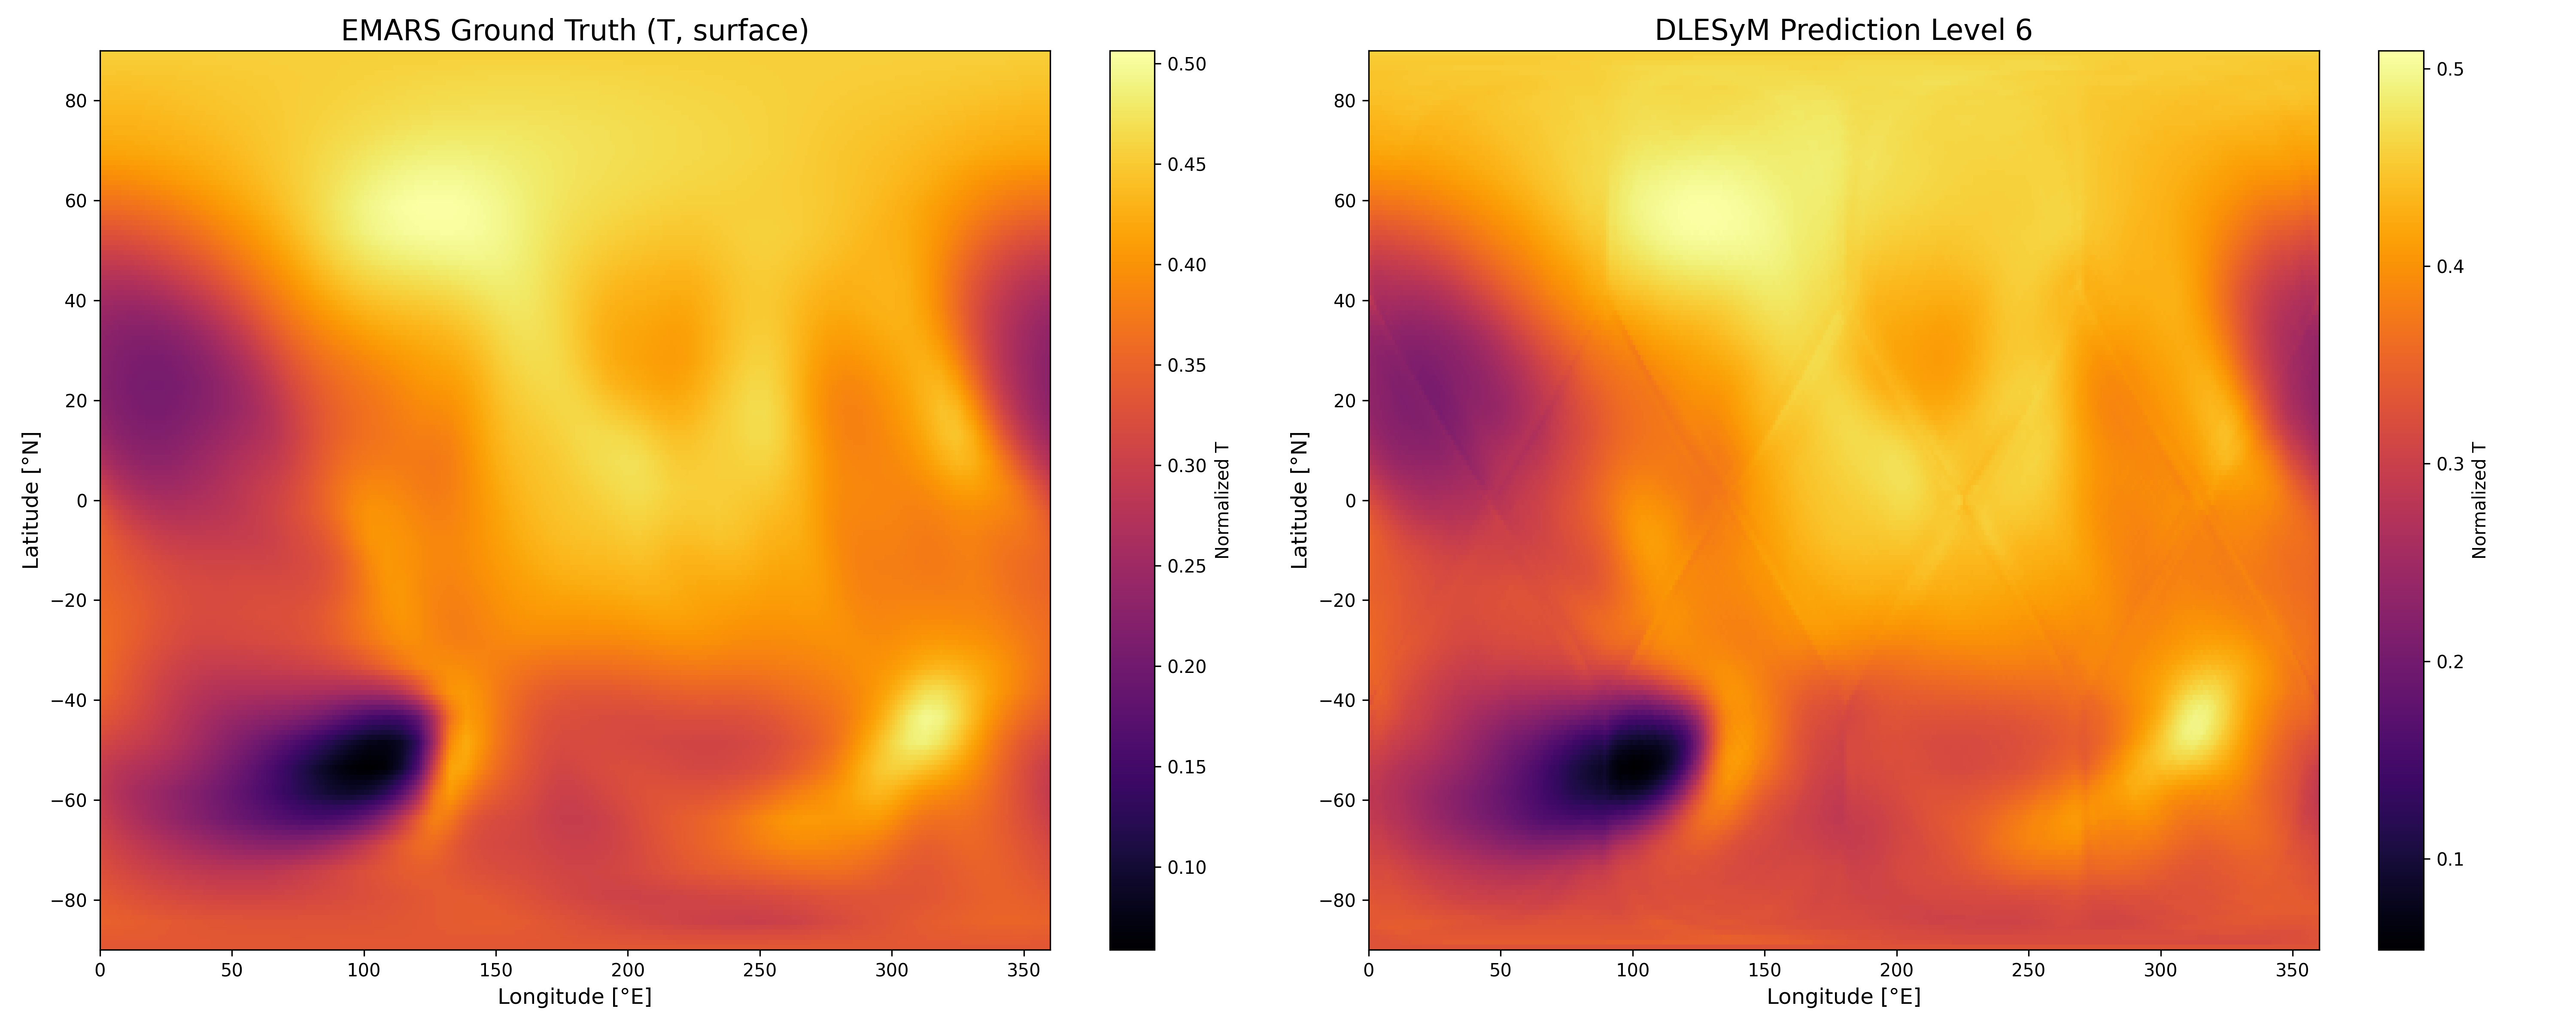
\includegraphics[width=\columnwidth]{dlesym_comparison_level6.png}
    \caption{Single-step prediction at HEALPix Level~6. Left: EMARS ground truth surface temperature. Right: DLESyM HEALPix U-Net prediction. Both panels show normalized temperature on a latitude--longitude projection.}
    \label{fig:comparison}
\end{figure}

\subsection{Recursive Rollout Stability}

A critical test for any weather emulator is whether it remains stable when predictions are fed back as inputs for multi-step forecasting. We evaluated the HEALPix U-Net by unrolling it autoregressively for 24 consecutive one-hour steps starting from a single initial condition.

Figure~\ref{fig:rollout_stability} shows the RMSE (computed on normalized temperature across all 28 vertical levels) as a function of forecast horizon. The error grows monotonically and smoothly from approximately 0.004 at T+1\,h to approximately 0.029 at T+24\,h. Crucially, the RMSE curve shows \textbf{no sign of divergence or exponential blowup} over the full 24-hour window. The growth rate decelerates after approximately 12 hours, suggesting that the model asymptotically approaches its internal climatology rather than producing unphysical states.

This 24-hour stable rollout represents a significant improvement over the baseline 3D U-Net, which exhibited forecast drift toward climatology by approximately 10 hours in preliminary experiments. The improvement is attributable to the HEALPix-aware padding, which prevents artificial discontinuities at face boundaries from amplifying during recursive application.

\begin{figure}[t]
    \centering
    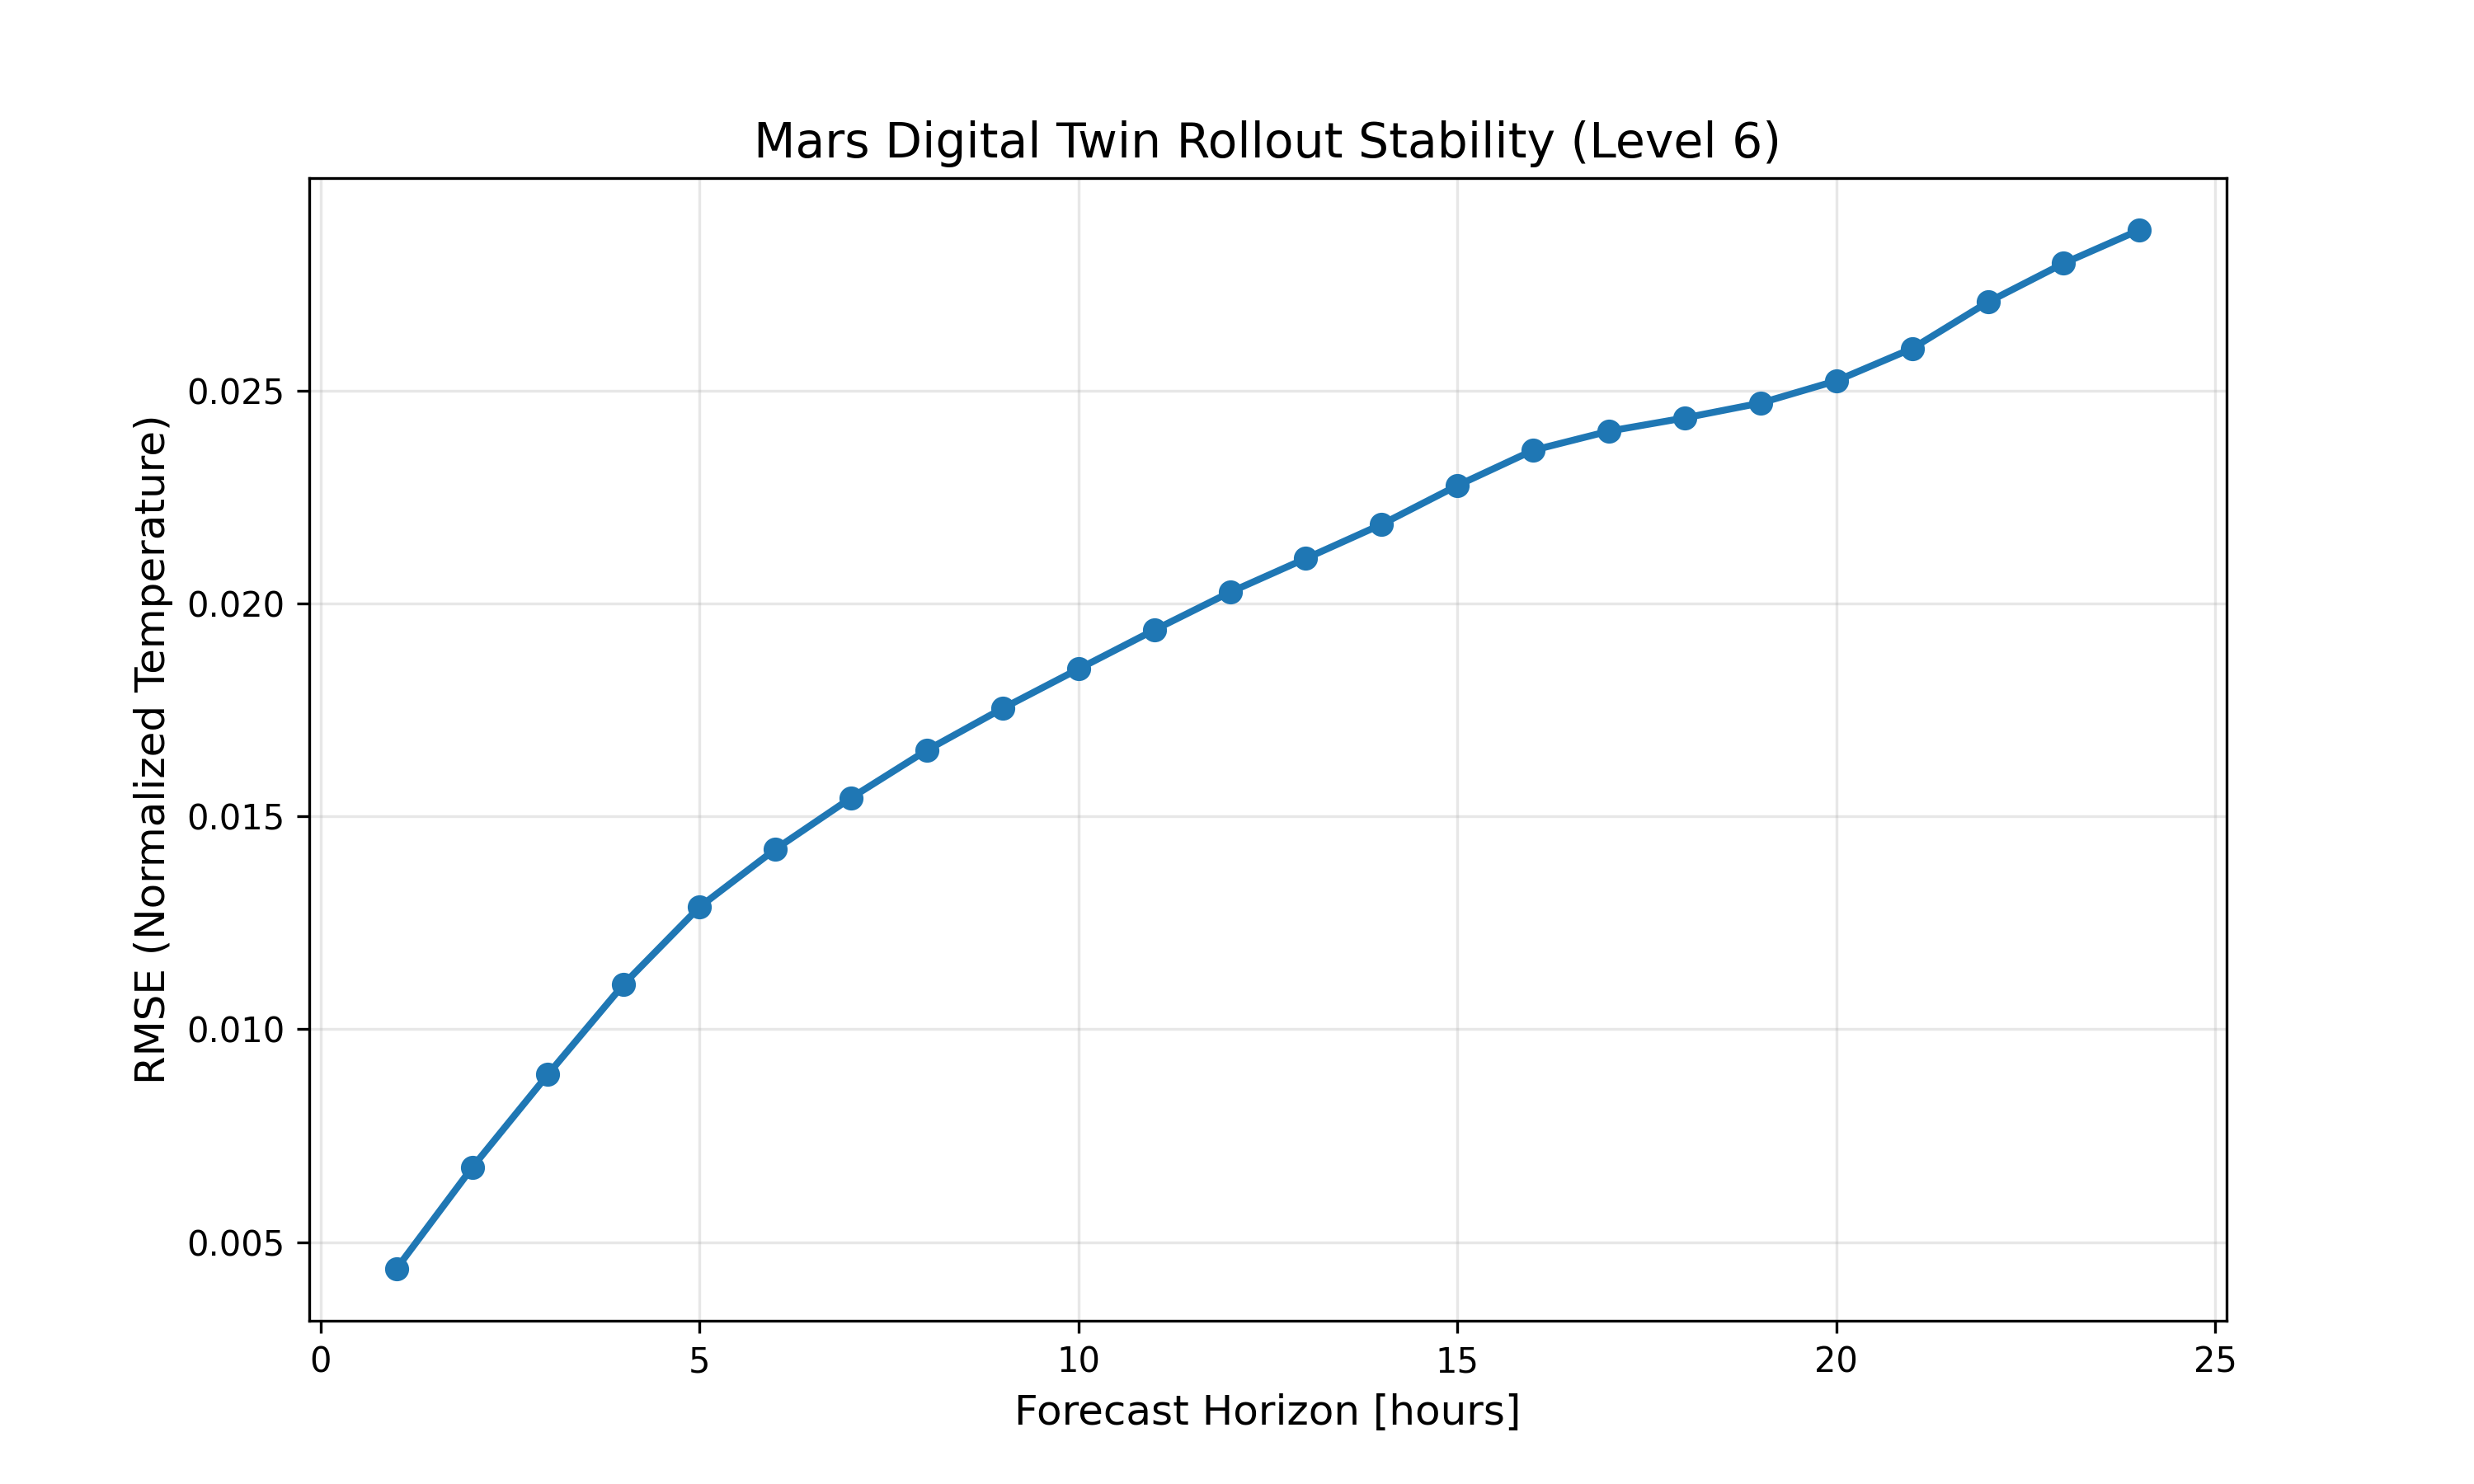
\includegraphics[width=\columnwidth]{rollout_stability_level6.png}
    \caption{Rollout stability over 24 forecast hours. RMSE of normalized temperature increases monotonically from ${\sim}0.004$ to ${\sim}0.029$ without divergence, demonstrating the model's ability to maintain physically coherent forecasts for a full Martian sol.}
    \label{fig:rollout_stability}
\end{figure}

Figure~\ref{fig:rollout_24h} compares the model's 24-hour forecast against the corresponding EMARS ground truth for surface temperature. Despite 24 recursive applications, the predicted field retains the correct large-scale thermal structure: the position and intensity of the southern polar vortex, the warm equatorial band, and mid-latitude gradients are all preserved. Diamond-shaped artifacts corresponding to HEALPix face boundaries are visible in the 24-hour prediction, indicating that the inter-face padding, while effective, introduces subtle imprints under repeated application. These artifacts represent an area for architectural improvement.

\begin{figure}[t]
    \centering
    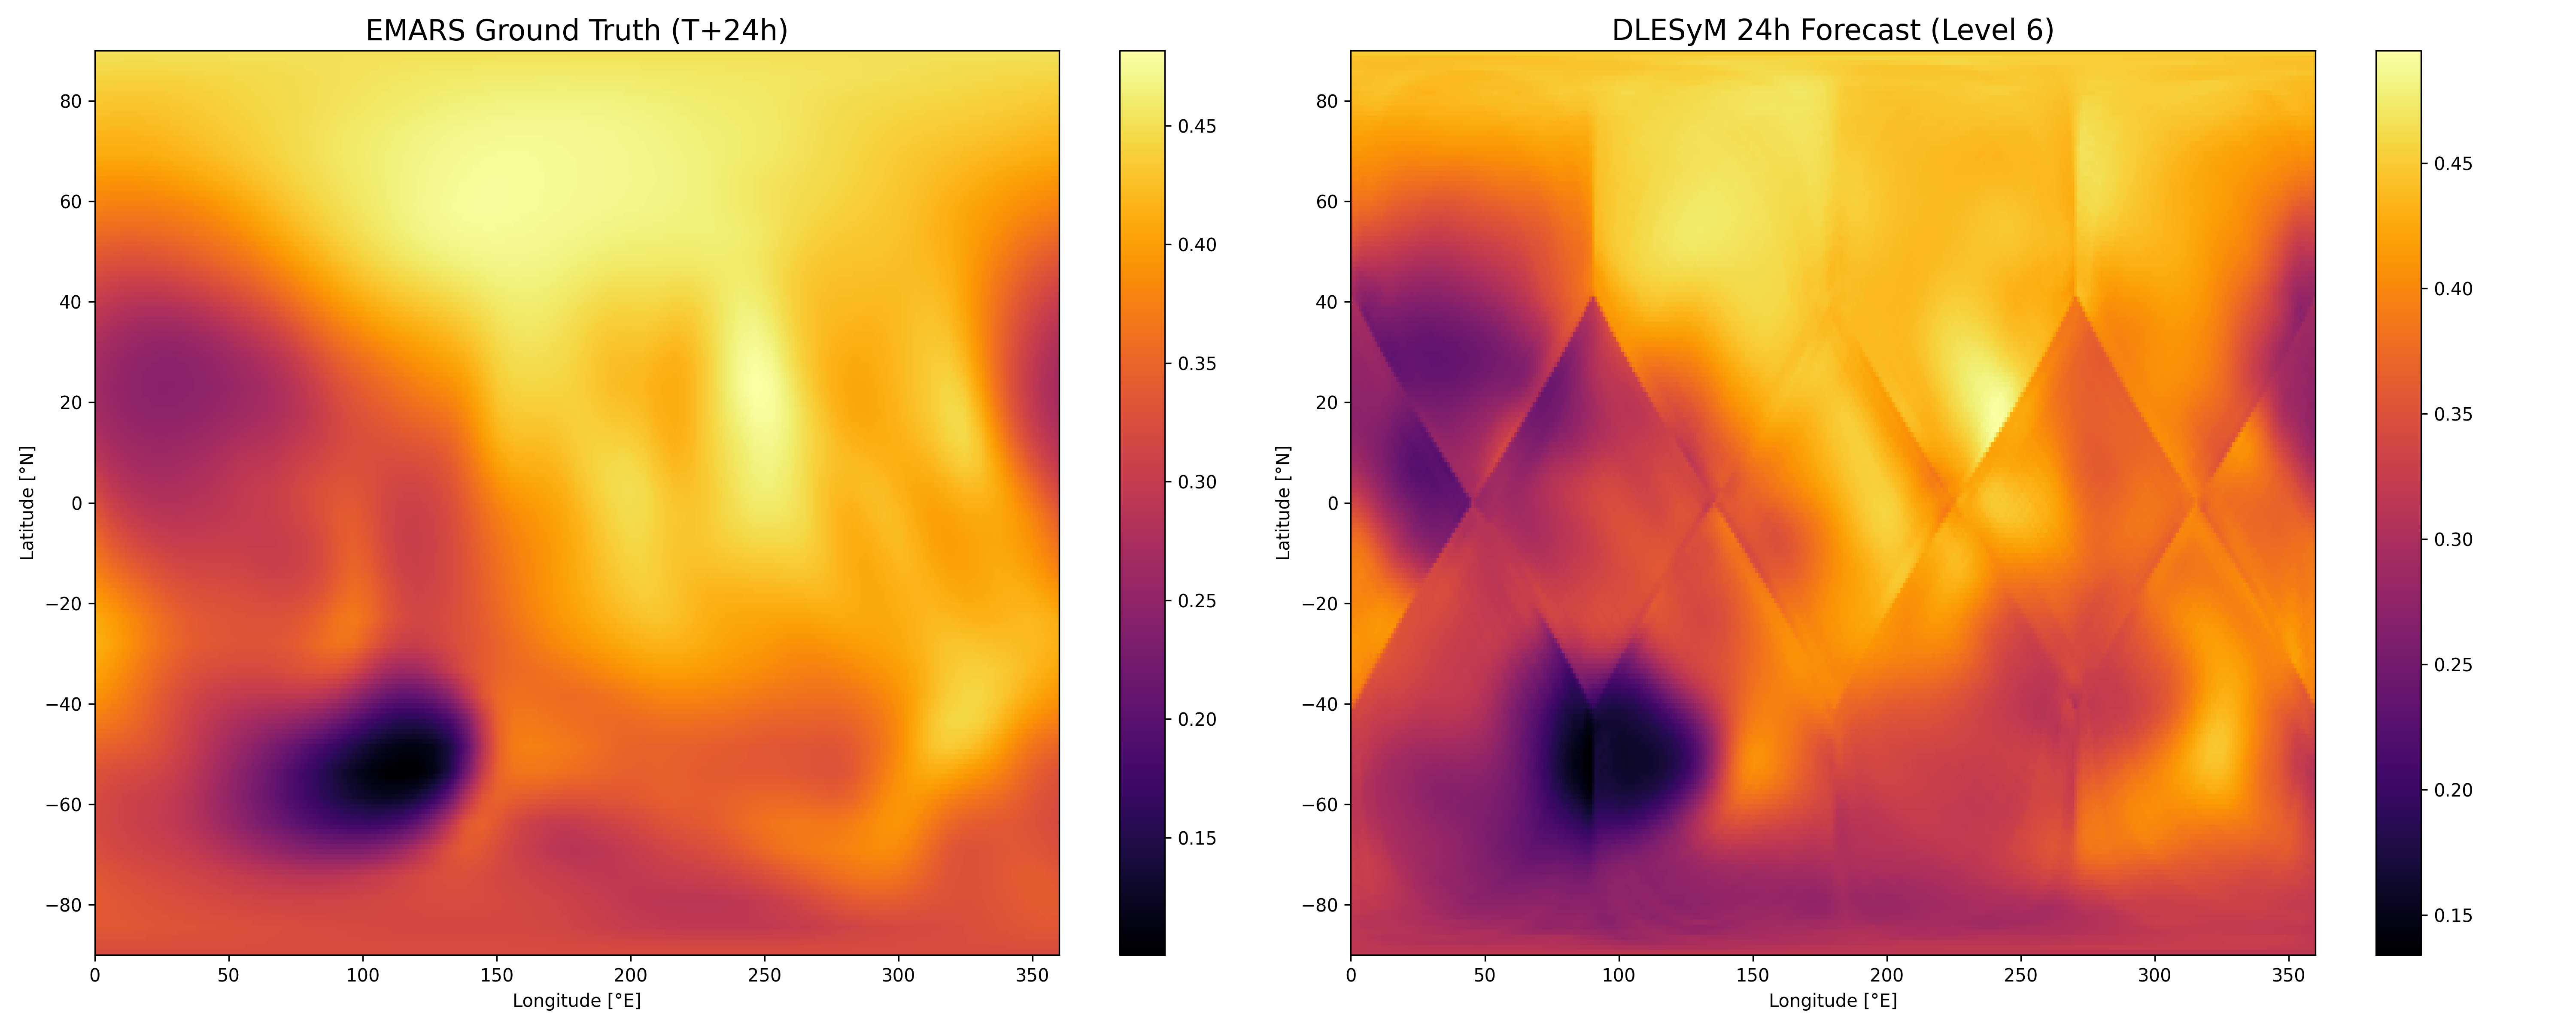
\includegraphics[width=\columnwidth]{rollout_comparison_24h_level6.png}
    \caption{24-hour rollout comparison. Left: EMARS ground truth at T+24\,h. Right: HEALPix U-Net prediction after 24 recursive steps. The model maintains realistic large-scale structures including the polar vortex and equatorial gradients, though faint HEALPix face-boundary artifacts emerge at long lead times.}
    \label{fig:rollout_24h}
\end{figure}

\subsection{Computational Efficiency}

The HEALPix U-Net generates a one-hour forecast in approximately 0.5~seconds on a single NVIDIA GPU. Producing a full 24-hour rollout requires roughly 12~seconds of wall-clock time. In contrast, integrating the GFDL/NASA Mars GCM at comparable resolution requires substantial HPC resources and orders-of-magnitude more time~\cite{haberle2019}. This speedup makes the deep-learning emulator suitable for generating large ensembles for mission risk assessment, where hundreds of potential scenarios can be simulated in minutes.

The model's compact size (4.3M parameters, ${\sim}$17~MB checkpoint) also makes it deployable on modest hardware, potentially even onboard future Mars-orbiting or surface platforms for real-time forecasting applications.

% ===================================================================
\section{Discussion}
% ===================================================================

\subsection{Architecture Benefits}

Our results confirm that respecting the geometry of the sphere during convolution yields substantial benefits for global weather emulation. The HEALPix-aware padding eliminates the artificial discontinuities that standard padding introduces at face boundaries. When the model is applied recursively, these discontinuities would otherwise amplify with each step, leading to the boundary artifacts and early divergence observed in naive approaches. The DLESyM-style architecture achieves better accuracy with 4.3M parameters than the 3D U-Net achieves with 30M, validating the principle that inductive biases aligned with the problem geometry can substitute for raw model capacity.

The Capped GELU activation~\cite{hendrycks2016} further contributes to rollout stability by preventing unbounded intermediate activations that can trigger numerical instability during long autoregressive chains.

\subsection{Limitations}

Several factors currently limit the model's performance and applicability.

\paragraph{Forecast horizon.} While the model remains stable for 24 hours, the RMSE at T+24\,h (${\sim}$0.029) is approximately seven times larger than at T+1\,h (${\sim}$0.004). Beyond ${\sim}$12 hours, the forecast increasingly reflects the model's learned climatology rather than the specific atmospheric evolution from the initial condition. Extending the useful forecast horizon likely requires incorporating temporal context (e.g., multiple input time steps or recurrent architectures) and additional prognostic variables.

\paragraph{Aerosol representation.} Dust is a primary driver of the Martian atmospheric thermal structure~\cite{montabone2015eight,kahre2017}. During global dust storms, radiative heating of the atmosphere changes drastically. Our model, which forecasts only $T$, $U$, and $V$, cannot anticipate these aerosol-driven regime transitions. Incorporating dust and water-ice opacity as additional channels is a critical next step.

\paragraph{Face-boundary artifacts.} The diamond-shaped imprints visible in the 24-hour forecast (Figure~\ref{fig:rollout_24h}) indicate that the HEALPixPadding, while substantially better than naive alternatives, does not perfectly reproduce spherical continuity. The blending strategy at three-face vertices uses simple 50/50 averaging, which may introduce subtle biases under repeated application. More sophisticated blending or learned padding strategies could mitigate this.

\paragraph{Reanalysis bias inheritance.} The model inherits biases from EMARS itself. Because EMARS assimilates observations from a limited number of local times (primarily corresponding to spacecraft overpasses), the diurnal cycle in the reanalysis may not be fully representative~\cite{greybush2019}. Future work could benefit from multi-model ensembles or physically-informed constraints enforcing conservation laws.

\subsection{Broader Implications}

By demonstrating that a parsimonious model can capture the core dynamics of a different planet's atmosphere, we validate the cross-planetary applicability of HEALPix-based architectures. Mars serves as a useful testbed: its lack of oceans and relatively simple surface isolate atmospheric behaviors that are often masked by complex oceanic interactions on Earth. Insights from the Martian digital twin---particularly regarding the minimum model complexity needed to represent atmospheric dynamics---could inform more efficient architectures for Earth climate emulators.

We envision a future system where a deep-learning digital twin is periodically updated with new spacecraft observations, allowing it to correct its forecasts toward the observed state, analogous to traditional Kalman filter-based systems but at a fraction of the computational cost.

% ===================================================================
\section{Conclusions}
% ===================================================================

We have presented a proof-of-concept deep-learning emulator for the Martian atmosphere that adapts the DLESyM HEALPix-aware convolutional framework to EMARS reanalysis data. Our key findings are:

\begin{enumerate}
    \item \textbf{Geometry matters.} A HEALPix-aware 2D U-Net with inter-face padding achieves validation MSE of $1.58 \times 10^{-5}$---more than an order of magnitude better than a standard 3D U-Net baseline---with fewer parameters (4.3M vs.\ 30M).

    \item \textbf{Stable long-range rollout.} The model produces physically coherent autoregressive forecasts for 24 hours with monotonically growing but bounded RMSE, extending the forecast horizon beyond the 10-hour limit of earlier approaches.

    \item \textbf{Extreme efficiency.} One-hour forecasts require ${\sim}$0.5~seconds on a single GPU, enabling ensemble forecasting for mission risk assessment at negligible computational cost compared to GCM integration.

    \item \textbf{Compact deployability.} The 17~MB model checkpoint opens possibilities for onboard forecasting on future Mars missions.
\end{enumerate}

While limitations regarding aerosol representation, face-boundary artifacts at long lead times, and reanalysis bias inheritance remain, the foundation laid here demonstrates that data-driven methods can capture the complex dynamical propagation of a non-terrestrial atmosphere. Future work will focus on incorporating aerosol dynamics, extending to multi-step input conditioning with recurrent units, exploring hybrid architectures coupling neural emulators with physical parameterizations, and validating against independent Mars atmospheric observations.

% ===================================================================
\section*{Acknowledgments}
% ===================================================================

We thank the Keck Institute for Space Studies (KISS) at the California Institute of Technology for organizing two workshops on ``Digital Twins for Solar System Exploration: Enceladus,'' which provided the insight, expertise, and discussions that inspired this research. We thank the EMARS development team for creating and maintaining the publicly available reanalysis dataset~\cite{greybush2019}. This study was inspired by the parsimonious deep-learning weather prediction model developed by Karlbauer et al.~\cite{karlbauer2024} and the DLESyM framework~\cite{wattmeyer2024}. We acknowledge the use of open-source packages including \texttt{earth2grid}~\cite{bonev2023spherical}, PyTorch~\cite{paszke2019pytorch}, and HEALPix~\cite{gorski2005healpix}. This work did not receive external funding.

% ===================================================================
% References
% ===================================================================

\bibliographystyle{unsrtnat}

\begin{thebibliography}{18}

\bibitem{wattmeyer2024}
Watt-Meyer, O., Dresdner, G., McGibbon, J., et al. (2024).
\newblock {ACE2}: Accurately learning the {E}arth's climatic variables from a coupled atmosphere model.
\newblock \textit{arXiv preprint arXiv:2310.02074}.

\bibitem{hendrycks2016}
Hendrycks, D. and Gimpel, K. (2016).
\newblock {G}aussian error linear units ({GELUs}).
\newblock \textit{arXiv preprint arXiv:1606.08415}.

\bibitem{liu2022convnext}
Liu, Z., Mao, H., Wu, C.-Y., Feichtenhofer, C., Darrell, T., and Xie, S. (2022).
\newblock A {ConvNet} for the 2020s.
\newblock In \textit{Proceedings of the IEEE/CVF Conference on Computer Vision and Pattern Recognition}, pp.\ 11976--11986.

\bibitem{ronneberger2015}
Ronneberger, O., Fischer, P., and Brox, T. (2015).
\newblock {U-Net}: Convolutional networks for biomedical image segmentation.
\newblock In \textit{International Conference on Medical Image Computing and Computer-Assisted Intervention}, pp.\ 234--241. Springer.

\bibitem{cicek20163d}
\c{C}i\c{c}ek, \"{O}., Abdulkadir, A., Lienkamp, S.~S., Brox, T., and Ronneberger, O. (2016).
\newblock {3D U-Net}: Learning dense volumetric segmentation from sparse annotation.
\newblock In \textit{International Conference on Medical Image Computing and Computer-Assisted Intervention}, pp.\ 424--432. Springer.

\bibitem{read2015physics}
Read, P.~L., Lewis, S.~R., and Mulholland, D.~P. (2015).
\newblock The physics of {M}artian weather and climate: A review.
\newblock \textit{Reports on Progress in Physics}, 78(12):125901.

\bibitem{haberle2019}
Haberle, R.~M., Clancy, R.~T., Forget, F., Smith, M.~D., and Zurek, R.~W., eds. (2017).
\newblock \textit{The Atmosphere and Climate of Mars}.
\newblock Cambridge University Press.

\bibitem{greybush2019}
Greybush, S.~J., Gillespie, H.~E., and Wilson, R.~J. (2019).
\newblock Transient eddies in the {TES/MCS} {E}nsemble {M}ars {A}tmosphere {R}eanalysis {S}ystem ({EMARS}).
\newblock \textit{Icarus}, 317:158--181.

\bibitem{greybush2012ensemble}
Greybush, S.~J., Wilson, R.~J., Hoffman, R.~N., Hoffman, M.~J., Miyoshi, T., Ide, K., McConnochie, T., and Kalnay, E. (2012).
\newblock Ensemble {K}alman filter data assimilation of {T}hermal {E}mission {S}pectrometer temperature retrievals into a {M}ars {GCM}.
\newblock \textit{Journal of Geophysical Research: Planets}, 117(E11).

\bibitem{karlbauer2024}
Karlbauer, M., Cresswell-Clay, N., Durran, D.~R., Moreno, R.~A., Kurth, T., Bonev, B., Brenowitz, N., and Butz, M.~V. (2024).
\newblock Advancing parsimonious deep learning weather prediction using the {HEALPix} mesh.
\newblock \textit{Journal of Advances in Modeling Earth Systems}, 16(8):e2023MS004021.

\bibitem{gorski2005healpix}
G\'{o}rski, K.~M., Hivon, E., Banday, A.~J., Wandelt, B.~D., Hansen, F.~K., Reinecke, M., and Bartelmann, M. (2005).
\newblock {HEALPix}: A framework for high-resolution discretization and fast analysis of data distributed on the sphere.
\newblock \textit{The Astrophysical Journal}, 622(2):759.

\bibitem{bi2023pangu}
Bi, K., Xie, L., Zhang, H., Chen, X., Gu, X., and Tian, Q. (2023).
\newblock {Pangu-Weather}: A 3{D} high-resolution model for fast and accurate global weather forecast.
\newblock \textit{Nature}, 619(7970):533--538.

\bibitem{lam2023graphcast}
Lam, R., Sanchez-Gonzalez, A., Willson, M., et al. (2023).
\newblock {GraphCast}: Learning skillful medium-range global weather forecasting.
\newblock \textit{Science}, 382(6677):1416--1421.

\bibitem{pathak2022fourcastnet}
Pathak, J., Subramanian, S., Harrington, P., et al. (2022).
\newblock {FourCastNet}: A global data-driven high-resolution weather forecasting model.
\newblock \textit{arXiv preprint arXiv:2202.11214}.

\bibitem{montabone2015eight}
Montabone, L., Forget, F., Millour, E., et al. (2015).
\newblock Eight-year climatology of dust optical depth on {M}ars.
\newblock \textit{Icarus}, 251:65--95.

\bibitem{kahre2017}
Kahre, M.~A., Murphy, J.~R., Newman, C.~E., Wilson, R.~J., Cantor, B.~A., Lemmon, M.~T., and Wolff, M.~J. (2017).
\newblock The {M}ars dust cycle.
\newblock In Haberle, R.~M. et al., eds., \textit{The Atmosphere and Climate of Mars}, pp.\ 295--337. Cambridge University Press.

\bibitem{bonev2023spherical}
Bonev, B., Kurth, T., Grossman, C., et al. (2023).
\newblock Spherical {F}ourier neural operators: Learning stable dynamics on the sphere.
\newblock In \textit{International Conference on Machine Learning}, pp.\ 2806--2823. PMLR.

\bibitem{paszke2019pytorch}
Paszke, A., Gross, S., Massa, F., et al. (2019).
\newblock {PyTorch}: An imperative style, high-performance deep learning library.
\newblock In \textit{Advances in Neural Information Processing Systems}, vol.\ 32.

\bibitem{kingma2015adam}
Kingma, D.~P. and Ba, J. (2015).
\newblock Adam: A method for stochastic optimization.
\newblock In \textit{Proceedings of the 3rd International Conference on Learning Representations (ICLR)}.

\end{thebibliography}

\end{document}
